% Copyright 2017 Justin Gombos
%
% Licensed under the Apache License, Version 2.0 (the "License");
% you may not use this file except in compliance with the License.
% You may obtain a copy of the License at
%
%     http://www.apache.org/licenses/LICENSE-2.0
%
% Unless required by applicable law or agreed to in writing, software
% distributed under the License is distributed on an "AS IS" BASIS,
% WITHOUT WARRANTIES OR CONDITIONS OF ANY KIND, either express or implied.
% See the License for the specific language governing permissions and
% limitations under the License.

\documentclass[pdftex,12pt,titlepage=false]{scrartcl}

\usepackage[table,dvipsnames,svgnames]{xcolor} % for LightGoldenrodYellow (loads also »colortbl«)
\usepackage[margin=20mm,bottom=10mm,pdftex,letterpaper]{geometry}
\usepackage[utf8]{inputenc}
\usepackage[T1]{fontenc} %suggested to avoid ``OT1 encoding''
\usepackage{hyperref}
\usepackage{array}
\usepackage[pdftex]{graphicx}
\usepackage{multicol}
\usepackage{multirow}
\usepackage{wrapfig}
\usepackage{soul}

\newcommand{\yesbad}{\textcolor{red}{yes}}
\newcommand{\nogood}{\textcolor{ForestGreen}{no}}
\newcommand{\yesgood}{\textcolor{ForestGreen}{yes}}
\newcommand{\nobad}{\textcolor{red}{no}}

\title{\rmfamily Configuring Outlook's built-in S/MIME Cryptosystem (Mac \& Windows)}
%\newcommand{\theauthor}{J.G.}
%\author{\rmfamily\theauthor}
\date{\rmfamily\today}

\newcommand{\comment}[1]{} %inline comment by gobbling the argument

\newcommand*{\fullref}[1]{\hyperref[{#1}]{\autoref*{#1} \nameref*{#1}}}

\newcommand{\secorio}{\href{https://www.secorio.com/}{
\includegraphics[width=2cm]{images/logo_comodo.png}\tiny via Secorio}}

\newcommand{\safaricaveat}{\tiny(Safari automatically installs S/MIME
  keys on a ``Keychain Access''-reachable keyring, which (according to
  \href{https://support.comodo.com/index.php?/Knowledgebase/Article/View/1177/37/apple-mail-and-outlook-for-os-x-smime-installation}{%
    Comodo docs} and
  \href{https://technet.microsoft.com/en-us/library/jj984223(v=office.16).aspx}{MS
    docs}), Outlook uses.}

\newcommand{\keystoreintl}{\tiny(browser uses its own internal key store)}

\begin{document}

\maketitle

\tableofcontents

\section{Prerequisites}\label{prereq}
\begin{itemize}
\item MS Outlook 2013 or later is recommended.  Earlier versions
  officially support S/MIME but users often report difficulties,
  particularly with Outlook 2010.
\item A browser is only needed initially to create SSL keys, and will
  not be used thereafter.  Any of these browsers will work:

  % Would be nice to use \rowcolors in the following table, but text
  % gets clobbered in the \multirow cell, and
  % \hiderowcolors is broken entirely.
  \begin{tabular}{lp{50mm}>{\small}p{0.37\textwidth}}
    \textsl{\textbf{Browser}}          & \textsl{\textbf{Key storage consistent with Outlook}} & \textsl{\textbf{Notes}}\\
    Chrome/Chromium \tiny(OS/X)        & \yesgood                & Some versions of Chrome may have problems with key generation.\\
    \hline
    Chrome/Chromium \tiny(Windows)     & \nobad\ \keystoreintl   & \multirow{2}{=}{Works but needs some extra steps (section~\ref{cert_install}) to copy keys.}\\
    \cline{1-2}
    Firefox \tiny(all platforms)       & \nobad\ \keystoreintl   & \\
    \hline
    \st{Internet Explorer \tiny(OS/X)} & --                      & Don't use IE on Mac; latest version (4.0) is discontinued.\\
    \hline
    Internet Explorer \tiny(Windows)   & \yesgood                & \\
    \hline
    Safari \tiny(OS/X)                 & \yesgood\ \safaricaveat & Some versions of Safari may have problems with key generation.\\
    \hline
    Safari \tiny(Windows)              & ? \tiny(undocumented, left as an exercise for the readers ;]) & \\
  \end{tabular}

  Browsers above that are indicated ``\yesgood'' for sharing the same
  key storage as Outlook are more convenient for this setup because
  keys need not be copied, thus section~\ref{cert_install} may be
  skipped.
\end{itemize}

\section{Instructional videos (optional)}
These videos are optional; not required by this guide.\\[0.5em]

\rowcolors{2}{Khaki}{LightGoldenrodYellow} %this breaks old versions of dvisvgm!
\begin{tabular}{llllp{0.4\textwidth}}
  \slshape\textbf{Link} & \slshape\textbf{Outlook ver.} & \slshape\textbf{Browser ver.} & \slshape\textbf{CA} & \slshape\textbf{Scope + Notes}\\
  \href{https://www.youtube.com/watch?v=6OxOo-w3Ymo}{6OxOo-w3Ymo}
  & 2007 & n/a & n/a &\\
  \href{https://www.youtube.com/watch?v=wGHaB0elkaA}{wGHaB0elkaA}
  & 2010 & Firefox & Symantec & Demonstrates how to use Firefox and manually copy the key pair into Outlook.\\
  \href{https://www.youtube.com/watch?v=n3rOEpGjrc}{n3rOEpGjrc}
  & 2013 & Chrome & Comodo & \\
  \href{https://www.youtube.com/watch?v=sfancZGEGjg\&start=535}{sfancZGEGjg}
  & 2013-2016 & IE? & Comodo & This comprehensive video covers every step in this entire document.  It demonstrates a case where the browser automatically installs the key where Outlook can find it.  The first 9 min. of the video is blather, but the link supplied skips to the relevant part.\\
  \href{https://www.youtube.com/watch?v=4fmBzeq8BVA}{4fmBzeq8BVA}
  & 2016 & IE? & Entrust & Outlook had automatic visibility to the key in this demo on Windows, so IE was likely used.\\
\end{tabular}

\section{Prep to receive encrypted mail or to send signed mail}
% \subsection{YouTube video (alternative to this document)}
% For Outlook 2013 and 2016 users there is a comprehensive YouTube video
% demonstrating whole process using Comodo for the certificate
% authority.  It starts with nine minutes of blather, but {\large
%   \href{https://www.youtube.com/watch?v=sfancZGEGjg\&start=535}{this
%     link}} skips straight to the relevant part.  That video is
% detailed enough to replace this entire document.

\subsection{Get an S/MIME certificate}\label{catable}
In your browser go to one of these certificate authorities (\textbf{Justin recommends Comodo via Secorio}):\\

\rowcolors{2}{Khaki}{LightGoldenrodYellow} %this breaks old versions of dvisvgm!
\begin{tabular}{lp{2.3cm}l>{\tiny}p{0.36\textwidth}}
  \slshape\textbf{certificate authority} (``CA'')
  & \slshape\textbf{price} \newline\tiny(for non-commercial individual use)
  & \slshape\textbf{validity}
  & \slshape\normalsize\textbf{notes}\\
  %\hline\\
  \href{https://www.cacert.org/}{
\includegraphics[width=2cm]{images/logo_cacert4.png}} & gratis & 6|24 mos.\tiny (\href{http://wiki.cacert.org/FAQ/Privileges}{criteria}) & community driven; getting a 2yr cert requires meeting w/someone and showing state-issued proof of id\\
  \href{https://secure.comodo.com/products/frontpage?area=SecureEmailCertificate}{
\includegraphics[width=2cm]{images/logo_comodo.png}\tiny direct} & gratis & 1 yr &\\
  \href{https://www.instantssl.com/ssl-certificate-products/free-email-certificate.html}{
\includegraphics[width=2cm]{images/logo_comodo.png}\tiny via InstantSSL} & gratis & 1 yr &\\
  \secorio & gratis & 1 yr & simple; assumed choice by this guide\\
  \href{https://www.entrust.com/secure-email-certificates/}{
\includegraphics[width=2cm]{images/logo_entrust.png}} & $\geq$\$20 & &\\
  \href{https://www.identrust.com/certificates/trustid.html}{
\includegraphics[width=2cm]{images/logo_trustid.png}} & $\geq$\$19 & &\\
  \href{https://www.startcomca.com/}{
\includegraphics[width=2cm]{images/logo_startcom.png}} & gratis & 2 yrs & distrusted by Mozilla and others, thus signed msgs will likely be seen as invalid unless recipients manually add Startcom's CA key to their keystore\\
  \href{https://buy.wosign.com/free/}{
\includegraphics[width=2cm]{images/logo_wosign.png}} & \st{gratis} n/a & \st{2 yrs} n/a & recently \textbf{discontinued} but still maintained in this list because they intend to return to business\\
\end{tabular}\\

% geotrust, symantec, thawte have discontinued service
% (the "\par" at the end of this ensures that the linespacing is sensible)
{\tiny Warning: the CAs that participate in e-mail certificate
  verification are constantly changing.  Many CAs have discontinued
  e-mail certification prior to this guide.  Those with no intent to
  return to service are omitted here, but some of the above listings
  are likely to become obsolete as this guide ages.  Consequently it
  might be interesting to check out the catalog of certificate
  authorities listed at
  \url{http://kb.mozillazine.org/Getting_an_SMIME_certificate}).\par}

\subsubsection{If you chose ``Comodo via Secorio''}
\begin{multicols}{2}
  \begin{enumerate}
  \item (secorio.com) If you are using the \emph{noscript} firefox
    plugin, you must enable javascript for \texttt{secorio.com} and
    \texttt{comodo.com}.
  \item (secorio.com) In the left frame, select ``\texttt{S/MIME Class
      2}'' (even though it's \emph{class 1} that we need), then click
    ``\texttt{Order}''.
  \item (secorio.com) Scroll down to ``\texttt{S/MIME Certificates}''
    and choose ``1 year'' in the pull-down to the right of the
    \emph{class 1} row.
  \item (comodo.com) Fill out the form that appears in a new tab.
    Setting a revocation password is optional (and it's a good
    idea).% Untick the
    % ``Comodo newsletter opt in'' crap (if it's there).
  \item (your inbox) An e-mail will arrive.  If your e-mail client
    renders it graphically, click the button ``\texttt{Click \&
      Install Comodo Email Certificate}''.  For text clients, follow
    the instructions in the e-mail.  If your mail client does not
    automatically use Firefox or IE to open URLs, right-click that
    button instead, copy the URL, and paste it in the address bar to
    force it to render in Firefox or IE.
  \item Skip to section~\ref{cert_install}
  \end{enumerate}
\end{multicols}

\subsubsection{If you chose another certificate authority}
Simply follow the instructions on the website of the CA.  It will
generally involve filling out a form and confirming an e-mail.

\subsection{Installing your certificate into Outlook}\label{cert_install}
If you created your key using a browser that uses the same key storage
as Outlook (as indicated \fullref{prereq}), skip to
\fullref{outlookcfg}.

\subsubsection{(Chrome only) Export your key from your browser}
There are multiple browsers which do not share the same key storage as
Outlook, but this section presumes you are using Chrome.  Follow
\href{https://www.youtube.com/watch?v=n3rOEpGjrc\&start=310}{YouTube
  video n3rOEpGjrc} (the link of which jumps you to the relevant point
in the video), or follow these steps:

\begin{minipage}{\textwidth}% This minipage inhibits page splitting
\begin{multicols}{2}
  \begin{enumerate}
  \item After creating the certificate (previous section) Chrome
    presents a status bar under the address bar saying ``Successfully
    stored client certificate..''.  Click the ``\texttt{View}'' button
    on that bar.
  \item There is a pop-up which showing basic information about your
    certificate.  Switch to the \texttt{Details} tab.
  \item Click the ``\texttt{Copy to File}'' button to launch an export
    wizard.
  \item Click \texttt{Next}.
  \item You are asked if you want to export the private key with the
    certificate.  The default answer is no, but you need to click
    ``\textbf{\texttt{yes}}'', then \texttt{Next}.
  \item You are asked which format to use.  Choose \texttt{PKCS\#12},
    then \texttt{Next}.
  \item You will be prompted for a password for the backup file.  A
    weak password is fine, because this backup file will not be
    transmitted or retained for long.  You will import it into Outlook
    locally, and then you will delete the backup file.
  \end{enumerate}
\end{multicols}
\end{minipage}

\vspace{1em}
Then skip to section~\ref{import} for steps to import the key into
Outlook.

\subsubsection{(Firefox only) Export your key from your browser}
There are multiple browsers which do not share the same key storage as
Outlook, but this section presumes you are using Firefox.  Watch
\href{https://www.youtube.com/watch?v=wGHaB0elkaA\&start=226}{YouTube
  video wGHaB0elkaA} or follow the steps below to export the key from
the Firefox and then import it into Outlook.

The video demonstrates using Outlook 2010 for the mail client and
Firefox (a pre-2012 version) for the browser.  The first few minutes
start by walking through key creation on Symantec's website, which is
useless because Symantec no longer offers the service.  So the YouTube
link skips that portion of the video automatically.
% Note that the speaker elects to use the (now obsolete) hash
% algorithm SHA-1.  Ignore that advice and just go with the default.

If not following the above-mentioned video, these are the steps to
export from a more recent version of Firefox:

\begin{enumerate}
  \item Go to: menu ($\equiv$) $\gg$ Options/Preferences $\gg$ Advanced
  $\gg$ Certificates $\gg$ View Certificates $\gg$ Your Certificates.\\[1em]%
  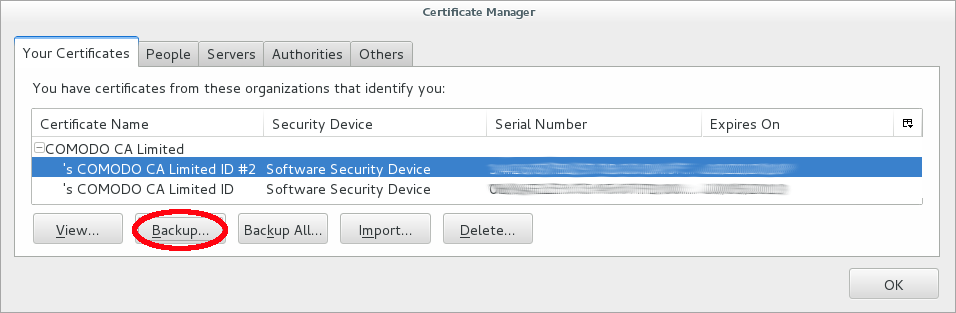
\includegraphics[width=0.7\textwidth]{images/firefox_cert_settings.png}
\item Highlight the line showing your new key.  It will be under the
  name of the CA you chose (e.g. the line under ``COMODO CA Limited''
  if you chose Comodo).
\item %\raisebox{0.6\baselineskip}{\parbox[t]{0.9\textwidth}{%
      %\begin{wrapfigure}{r}{0.7\textwidth}%
      %  \includegraphics[width=0.7\textwidth]{mailapp_firefox_cert_settings.png}
      %\end{wrapfigure}
  Click ``\texttt{Backup...}'' to export the key.
\item Save the file somewhere with a filename of your choice.  It will
  likely be given a \verb|.p12| extension.
\item\label{makebupw} You will be prompted for a password for the
  backup file.  A weak password is fine, because this backup file will
  not be transmitted or retained for long.  You will import it into
  Outlook locally, and then you will delete the backup file.
\end{enumerate}

\subsubsection{Import your key into Outlook}\label{import}
\begin{minipage}[t]{0.47\textwidth}
  \centerline{\textsl{(on OS/X)}} Simply double-click the
  \texttt{.p12} backup file that was produced in the previous section.
  OS/X will then import the key into the ``Keychain Access'' tool.
  According to
  \href{https://technet.microsoft.com/en-us/library/jj984223(v=office.16).aspx}{MS
    docs} Outlook 2016 uses Keychain Access.

  Older versions of Outlook may require more steps.  Outlook 2011
  users should read
  \href{https://support.microsoft.com/en-us/help/2957671/you-cannot-manage-your-certificates-in-the-mac-os-x-10-9-keychain}{%
    this doc}.
\end{minipage}\hfill%
\begin{minipage}[t]{0.47\textwidth}
  \centerline{\textsl{(on Windows)}}
  Watch
  % these are actually the config steps -- probably should be in the next section!
  % \href{https://www.youtube.com/watch?v=4fmBzeq8BVA\&start=107}{YouTube
  % video 4fmBzeq8BVA} (the link of which jumps you to the relevant
  % point in the video)
  \href{https://www.youtube.com/watch?v=n3rOEpGjrc\&start=390}{YouTube
    video n3rOEpGjrc} (the link of which jumps you to the relevant
  point in the video)
  or follow the steps below to import your key into Outlook 2013.
  \begin{enumerate}
  \item Go to File $\gg$ Options $\gg$ Trust Center (left pane) $\gg$
    Trust Center Settings..
  \item Go to Email Security (left pane) $\gg$ Digital IDs
    (Certificates) $\gg$ ``\texttt{Import/Export}'' (button)
  \item Click ``\texttt{Browse..}'' (button)
  \item Select the backup file that was produced in the previous
    section.
  \item In the ``\texttt{Password}'' field enter the password that was
    chosen in final step of the previous.
  \item Click ``\texttt{OK}'' in the pop-up dialog and the next
    window.
    % these are actually the config steps -- probably should be in the next section!
    % \item Go to Email Security (left pane) $\gg$ Settings.. (button)
    % \item Choose an arbitrary name for the field \texttt{Security Settings Name} (e.g. ``Comodo'')
    % \item Tick the box for ``\texttt{Default Security Settings for this cryptographic message format}''
    % \item Click ``\texttt{Choose..}'' to the right of ``\texttt{Signing Certificate}''
    % \item You'll likely only have one key, and it will be selected automatically.  Otherwise select the most recent key, and click ``\texttt{OK}''
  \item After the key is imported into Outlook, you should delete the
    backup file.  (You can always create a new backup file from
    Firefox if needed).
\end{enumerate}
\end{minipage}

\subsection{Configuring Outlook}\label{outlookcfg}
\begin{minipage}[t]{0.48\textwidth}
  \centerline{\textsl{(on OS/X)}}
  \begin{enumerate}
  \item On the Tools menu, click Accounts.
  \item Click the account that you want to send a digitally signed message from, click Advanced, and then click the Security tab.
  \item Under Digital signing, on the Certificate pop-up menu, click the certificate that you want to use.
  \end{enumerate}
\end{minipage}\hfill%
\begin{minipage}[t]{0.48\textwidth}
  \centerline{\textsl{(on Windows)}}\vspace{0.5em}Follow
  \href{https://www.ablebits.com/office-addins-blog/2014/04/11/email-encryption-outlook/#setup-email-certificate}{this
    document}.  That link skips the top portion and takes you straight
  to ``How to set up your e-mail certificate in Outlook'' because you
  already have a ``digital ID''.  That will configure Outlook for
  using your certificate.
\end{minipage}

% That process assumes Outlook already has your key automatically, and
% thus no export/import are needed.  If there are no issues with the key
% assignment step (that is, you were able to find your Comodo key), then
% you can skip to section~\ref{distribution}.

\subsection{Distribute your S/MIME certificate (aka public key)}\label{distribution}
In short: simply send an e-mail to the recipient using Outlook, and sign the message.\\

Detailed explanation: You have a pair of keys (these were created in
\fullref{catable}).  One is a public key and the other is a private
key.  The public key must be sent to those who will send you encrypted
e-mail.  They will use your public key to encrypt messages to you.
Your public key is automatically contained in the signature of all
messages you sign.

So to distribute your public key, simply send the other party an
signed e-mail from Outlook.  Encrypting this key distribution message
is optional, but it must be signed.  They can then extract your public
key from your signature.

\section{Prep to send encrypted mail% or verify signatures on received mail
}
Before you can send someone an encrypted message, you need the
recipients S/MIME certificate (public key).  This will normally come
to you when they send you a signed message, at which point you can
extract the certificate.  The certificate must then be associated to
that person in your address book.

\end{document}
